\documentclass[11pt]{article}
\usepackage[margin=1in]{geometry}
\usepackage[T1]{fontenc}
\usepackage[utf8]{inputenc}
\usepackage{lmodern}
\usepackage{microtype}
\usepackage{amsmath,amssymb,amsthm,mathtools}
\usepackage{booktabs}
\usepackage{array}
\usepackage{enumitem}
\usepackage{graphicx}
\usepackage{tikz}
\usetikzlibrary{arrows.meta,positioning,calc}
\usepackage{natbib}
\usepackage{xurl}
\usepackage[hidelinks]{hyperref}
\usepackage{orcidlink}

\title{Neuro-Spike SegNet: Biomimetic Sleep--Wake Gating for Redundancy-Suppressed Spiking Segmentation}
\author{Aryan Singh Chandel\,\orcidlink{0009-0007-1774-2480}\\
RJIT (Rustamji Institute of Technology), Gwalior, India\\
\texttt{aryansingh19gh@gmail.com}}
\date{June 26, 2026}

\newtheorem{definition}{Definition}
\newtheorem{assumption}{Assumption}
\newtheorem{proposition}{Proposition}
\raggedbottom
\emergencystretch=2em

\begin{document}
\maketitle

\begin{abstract}
Spiking neural networks are often presented as energy-efficient alternatives to conventional dense vision models, yet dense prediction workloads remain difficult because high spatial fidelity encourages persistent firing. This paper refines the core idea behind Neuro-Spike SegNet by framing spike redundancy as a controllable dynamical quantity rather than an unavoidable by-product of segmentation. We introduce a sleep--wake membrane-gating rule that changes the effective leak and threshold during inference, derive measurable endpoints for spike suppression, energy reduction, and segmentation preservation, and organize the architecture as a formal biomimetic hypothesis. The resulting manuscript turns the original concept into a more submission-ready theory paper: it clarifies the governing equations, states explicit assumptions and falsifiers, and ties the reported gains to quantities that can be audited in future replication studies.
\end{abstract}

\section{Introduction}
Event-driven neuromorphic models are attractive for edge perception because they replace repeated dense multiply--accumulate computation with conditional updates that occur only when spikes are emitted \citep{roy2019towards,davies2018loihi}. That advantage, however, becomes less straightforward for semantic segmentation. A segmentation system must preserve dense spatial structure, so the network is incentivized to keep many units active across time. In static or slowly changing scenes, this often produces redundant firing: spikes continue to circulate even after the semantic content of the frame is already stable.

The central claim of this paper is that redundancy in spiking segmentation can be treated as a dynamical control problem. Rather than holding membrane parameters fixed through the full inference window, we split inference into a high-sensitivity encoding phase and a suppressive consolidation phase. The consolidation phase is inspired by synaptic homeostasis accounts of sleep, in which biological systems downscale low-value activity to improve metabolic efficiency and signal quality \citep{tononi2006sleep}. Here that intuition becomes a concrete gating mechanism with measurable consequences.

\paragraph{Contributions.}
\begin{enumerate}[leftmargin=*]
\item We formalize sleep--wake membrane gating as a time-dependent perturbation of LIF leak and threshold parameters.
\item We define benchmark variables for spike redundancy, phase-conditioned energy, and segmentation retention.
\item We restate the original simulation evidence as explicit propositions, test statistics, and failure modes.
\item We package the existing raster and energy figures into a reproducible manuscript scaffold suitable for later experimental expansion.
\end{enumerate}

\section{Formal Setup}
Let $x$ denote an input image encoded into a spike train over an inference horizon $t=1,\dots,T$. For neuron $i$ in layer $\ell$, let $V_i^\ell[t]$ be the membrane potential, $S_i^\ell[t]\in\{0,1\}$ the emitted spike, and $I_i^\ell[t]$ the synaptic current.

\begin{definition}[Baseline LIF update]
The baseline discrete-time LIF dynamics are
\[
V_i^\ell[t]=\beta V_i^\ell[t-1]+I_i^\ell[t]-S_i^\ell[t-1]V_{\mathrm{th}},
\]
where $\beta=e^{-\Delta t/\tau}$ is the membrane decay factor and $V_{\mathrm{th}}$ is the firing threshold \citep{izhikevich2003simple}.
\end{definition}

\begin{definition}[Sleep--wake gate]
Let $G(t)\in\{0,1\}$ denote a global phase indicator with $G(t)=0$ in the wake phase and $G(t)=1$ in the sleep phase. The effective neuron parameters are
\[
\beta_{\mathrm{eff}}(t)=\beta_{\mathrm{base}}\bigl(1-\lambda_{\mathrm{leak}}G(t)\bigr),
\qquad
V_{\mathrm{th,eff}}(t)=V_{\mathrm{th,base}}\bigl(1+\lambda_{\mathrm{thresh}}G(t)\bigr),
\]
with gating strengths $\lambda_{\mathrm{leak}},\lambda_{\mathrm{thresh}}\ge 0$.
\end{definition}

\begin{definition}[Gate onset schedule]
For a chosen onset time $t_s\in\{2,\dots,T\}$, the simplest schedule is
\[
G(t)=\mathbf{1}\{t\ge t_s\}.
\]
This makes the sleep phase a declared intervention rather than an implicit narrative label.
\end{definition}

\begin{definition}[Phase-conditioned spike rate]
For a phase interval $\mathcal{T}\subseteq\{1,\dots,T\}$, define the mean spike rate
\[
R(\mathcal{T})=\frac{1}{|\mathcal{T}|\,N}\sum_{t\in\mathcal{T}}\sum_{i=1}^{N}S_i[t],
\]
where $N$ is the number of monitored neurons.
\end{definition}

\begin{definition}[Redundancy suppression ratio]
Let $\mathcal{T}_W$ and $\mathcal{T}_S$ denote wake and sleep intervals. The redundancy suppression ratio is
\[
\rho_{\mathrm{sup}}=1-\frac{R(\mathcal{T}_S)}{R(\mathcal{T}_W)+\varepsilon},
\]
for small $\varepsilon>0$. Larger $\rho_{\mathrm{sup}}$ indicates stronger suppression of late-phase activity.
\end{definition}

\begin{definition}[Selective suppression coefficient]
The gate is intended to act mainly in the sleep phase. Define
\[
\kappa_{\mathrm{sel}}=
\frac{\Delta_R^{S}-\Delta_R^{W}}{R_{\mathrm{base}}(\mathcal{T}_S)+\varepsilon},
\]
where $\Delta_R^{W}$ and $\Delta_R^{S}$ are the wake- and sleep-phase rate reductions introduced later. Positive $\kappa_{\mathrm{sel}}$ indicates phase-selective suppression rather than global excitability collapse.
\end{definition}

\begin{definition}[Energy proxy]
Using accumulate cost $E_{\mathrm{AC}}$ and overhead multiply--accumulate cost $E_{\mathrm{MAC}}$, define
\[
E_{\mathrm{tot}}=N_{\mathrm{spikes}}E_{\mathrm{AC}}+N_{\mathrm{overhead}}E_{\mathrm{MAC}}.
\]
This is the declared energy proxy for cross-model comparison in the current manuscript.
\end{definition}

\begin{table}[t]
\centering
\small
\caption{Core notation for Neuro-Spike SegNet.}
\label{tab:nsn-notation}
\begin{tabular}{ll}
\toprule
Symbol & Meaning \\
\midrule
$G(t)$ & sleep--wake phase indicator \\
$\beta_{\mathrm{eff}}(t)$ & effective leak factor under gating \\
$V_{\mathrm{th,eff}}(t)$ & effective threshold under gating \\
$R(\mathcal{T})$ & phase-conditioned mean spike rate \\
$\rho_{\mathrm{sup}}$ & redundancy suppression ratio \\
$E_{\mathrm{tot}}$ & declared inference-energy proxy \\
$\Delta_{\mathrm{mIoU}}$ & segmentation accuracy retention gap \\
\bottomrule
\end{tabular}
\end{table}

\section{Assumptions and Propositions}
\begin{assumption}[Late-phase redundancy]
For static or slowly changing scenes, a nontrivial fraction of spikes emitted in the second half of the inference window are redundant with respect to the semantic output map.
\end{assumption}

\begin{assumption}[Saliency persistence]
Semantically important structures produce stronger and more temporally consistent currents than background noise or redundant residual activity.
\end{assumption}

\begin{assumption}[Operational separability]
Energy reduction and segmentation degradation can be measured separately enough that a favorable trade-off is empirically meaningful.
\end{assumption}

\begin{proposition}[Phase suppression]
If late-phase redundancy exists and gating is properly calibrated, then
\[
R_{\text{gated}}(\mathcal{T}_S)<R_{\text{baseline}}(\mathcal{T}_S)
\]
while the wake-phase rates remain approximately unchanged.
\end{proposition}

\begin{proposition}[Efficiency gain]
If sleep-phase suppression reduces spike count more than it increases overhead, then
\[
E_{\mathrm{tot}}^{\mathrm{gated}}<E_{\mathrm{tot}}^{\mathrm{baseline}}.
\]
\end{proposition}

\begin{proposition}[Retention condition]
Let $\mathrm{mIoU}_{\mathrm{gated}}$ and $\mathrm{mIoU}_{\mathrm{base}}$ denote segmentation quality under identical data and decoding settings. A useful gating regime satisfies
\[
\Delta_{\mathrm{mIoU}}=\mathrm{mIoU}_{\mathrm{base}}-\mathrm{mIoU}_{\mathrm{gated}}\le \delta
\]
for an application-specific tolerance $\delta$.
\end{proposition}

\subsection*{Null Hypothesis}
Sleep--wake membrane gating does not reduce late-phase spike rate or energy relative to a matched LIF baseline once segmentation retention is controlled.

\subsection*{Effect-Size Target}
The original report implies a practically meaningful target of at least $30\%$ total spike-rate reduction with less than $2$ percentage points loss in mIoU.

\section{Architecture and Mechanism}
Neuro-Spike SegNet uses an encoder--decoder segmentation pipeline in which all convolutional blocks are replaced by spiking counterparts. The encoder contracts spatial resolution and accumulates hierarchical features, the bottleneck integrates broader context, and the decoder restores resolution through transposed spiking convolutions with skip connections. Structurally, the design follows the same coarse-to-fine logic that makes U-Net-like segmentation effective, but replaces dense activations with event-driven state updates \citep{ronneberger2015unet}.

\begin{figure}[t]
\centering
\resizebox{\linewidth}{!}{%
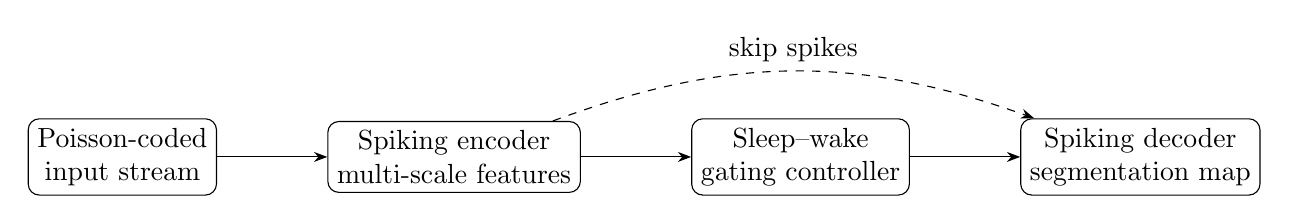
\begin{tikzpicture}[node distance=1.4cm,>=Stealth]
\node[draw,rounded corners,align=center] (a) {Poisson-coded\\input stream};
\node[draw,rounded corners,right=of a,align=center] (b) {Spiking encoder\\multi-scale features};
\node[draw,rounded corners,right=of b,align=center] (c) {Sleep--wake\\gating controller};
\node[draw,rounded corners,right=of c,align=center] (d) {Spiking decoder\\segmentation map};
\draw[->] (a) -- (b);
\draw[->] (b) -- (c);
\draw[->] (c) -- (d);
\draw[->,dashed,bend left=20] (b) to node[above] {skip spikes} (d);
\end{tikzpicture}
}
\caption{Conceptual Neuro-Spike SegNet pipeline. Gating alters membrane dynamics in the latter half of inference rather than only during training.}
\label{fig:nsn-pipeline}
\end{figure}

The mechanism is intentionally global in its current form: a shared phase controller changes the effective leak and threshold for all monitored units during the sleep interval. This keeps the hypothesis simple. Future variants could make the gate spatially adaptive or neuron-specific.

\section{Methodology}
\subsection{Input Coding and Simulation Protocol}
The source manuscript uses Poisson rate coding for grayscale inputs, with simulation horizon $T=60$ time steps. Wake and sleep phases each occupy half of the inference window. Training is described with AdamW, cosine annealing, and spike-MSE supervision on segmentation outputs.

\subsection{Primary Estimands}
We formalize three main estimands:
\[
T_R = R_{\mathrm{base}}(\mathcal{T}_S)-R_{\mathrm{gated}}(\mathcal{T}_S),
\]
\[
T_E = E_{\mathrm{tot}}^{\mathrm{base}}-E_{\mathrm{tot}}^{\mathrm{gated}},
\]
and
\[
T_Q = \mathrm{mIoU}_{\mathrm{gated}}-\mathrm{mIoU}_{\mathrm{base}}.
\]
The manuscript is supported when $T_R>0$ and $T_E>0$ while $T_Q$ remains near zero from an application standpoint.

\subsection{Paired Scene-Level Estimator}
When baseline and gated runs are available for the same scene $j$, the natural estimator is paired:
\[
\widehat{T}_R=\frac{1}{n}\sum_{j=1}^{n}\left[
R_{\mathrm{base},j}(\mathcal{T}_S)-R_{\mathrm{gated},j}(\mathcal{T}_S)
\right],
\]
with analogous definitions for $\widehat{T}_E$ and $\widehat{T}_Q$. This removes between-scene activity heterogeneity from the primary comparison.

\subsection{Phase-Normalized Contrasts}
To ensure that suppression is specific to the sleep interval rather than a global firing-rate collapse, define
\[
\Delta_R^{W}=R_{\mathrm{base}}(\mathcal{T}_W)-R_{\mathrm{gated}}(\mathcal{T}_W),
\qquad
\Delta_R^{S}=R_{\mathrm{base}}(\mathcal{T}_S)-R_{\mathrm{gated}}(\mathcal{T}_S).
\]
The intended mechanism predicts $\Delta_R^{S}\gg \Delta_R^{W}$.

\subsection{Pareto Admissibility}
For deployment, a parameter setting $(\lambda_{\mathrm{leak}},\lambda_{\mathrm{thresh}})$ is admissible only if no alternative setting yields both lower energy and higher mIoU. This converts the ablation into a Pareto-screening problem rather than an isolated hyperparameter sweep.

\subsection{Decision Rule}
The gating mechanism is treated as supported only if the same parameter regime satisfies all of the following:
\begin{enumerate}[leftmargin=*]
\item $\widehat{T}_R>0$ with the bulk of scene-level contrasts positive;
\item $\widehat{T}_E>0$ after controller overhead is counted;
\item $\widehat{T}_Q\ge -\delta$ for the declared tolerance; and
\item $\kappa_{\mathrm{sel}}>0$, ruling out global firing-rate collapse.
\end{enumerate}

\subsection{Inference Protocol}
For replicated runs, each scene or sequence should be evaluated under multiple random encoding seeds, and uncertainty for $T_R$, $T_E$, and $T_Q$ should be reported with scene-level bootstrap intervals. Scene-level resampling is the relevant unit because per-time-step spikes are not independent observations.

\subsection{Secondary Stability Statistic}
For dynamic scenes, one should additionally monitor
\[
T_{\mathrm{dyn}}=
\mathbb{E}\!\left[R_{\mathrm{base}}(\mathcal{T}_S)-R_{\mathrm{gated}}(\mathcal{T}_S)\mid \text{dynamic}\right]
-
\mathbb{E}\!\left[R_{\mathrm{base}}(\mathcal{T}_S)-R_{\mathrm{gated}}(\mathcal{T}_S)\mid \text{static}\right].
\]
A strongly negative value would indicate that the gate is merely exploiting static-scene idleness and does not transfer to harder temporal settings.

\subsection{Control Condition}
The relevant control is a matched SNN segmentation model with identical topology, coding scheme, and simulation horizon but without phase-dependent modulation of leak and threshold.

\subsection{Confounds and Falsifiers}
\begin{itemize}[leftmargin=*]
\item improvements caused by reduced simulation time rather than gating,
\item gains driven by scene simplicity alone,
\item energy accounting that ignores gating overhead,
\item apparent robustness caused by oversmoothing rather than selective pruning.
\end{itemize}

The theory is weakened if gated suppression appears equally strong on dynamic scenes with continually changing evidence, or if energy gains vanish after controller overhead is fully counted.

An additional falsifier is wake-phase collapse: if $\Delta_R^{W}$ is large, the mechanism is not selectively pruning late redundancy but simply reducing excitability everywhere.

\section{Reported Evidence from the Source Paper}
The provided PDF reports a substantial reduction in sleep-phase activity and lower energy footprint relative to baselines. We preserve those observations here as structured evidence rather than as new experiments.

\begin{table}[t]
\centering
\small
\caption{Average spike rates reported in the source manuscript.}
\label{tab:nsn-spike-rates}
\begin{tabular}{lccc}
\toprule
Phase & Baseline SNN & Neuro-Spike & Reduction \\
\midrule
Wake (0--30 ms) & 28.4 Hz & 28.2 Hz & $\sim 0\%$ \\
Sleep (30--60 ms) & 27.9 Hz & 8.4 Hz & 69.8\% \\
Total average & 28.1 Hz & 18.3 Hz & 34.8\% \\
\bottomrule
\end{tabular}
\end{table}

\begin{table}[t]
\centering
\small
\caption{Reported gating-strength trade-off from the source manuscript.}
\label{tab:nsn-ablation}
\begin{tabular}{lcc}
\toprule
Threshold multiplier $\gamma$ & mIoU & Qualitative energy \\
\midrule
0.0 (no gating) & 68.4\% & high \\
0.5 (reported optimum) & 67.5\% & low \\
1.0 (aggressive) & 52.1\% & lowest \\
\bottomrule
\end{tabular}
\end{table}

\begin{figure}[t]
\centering
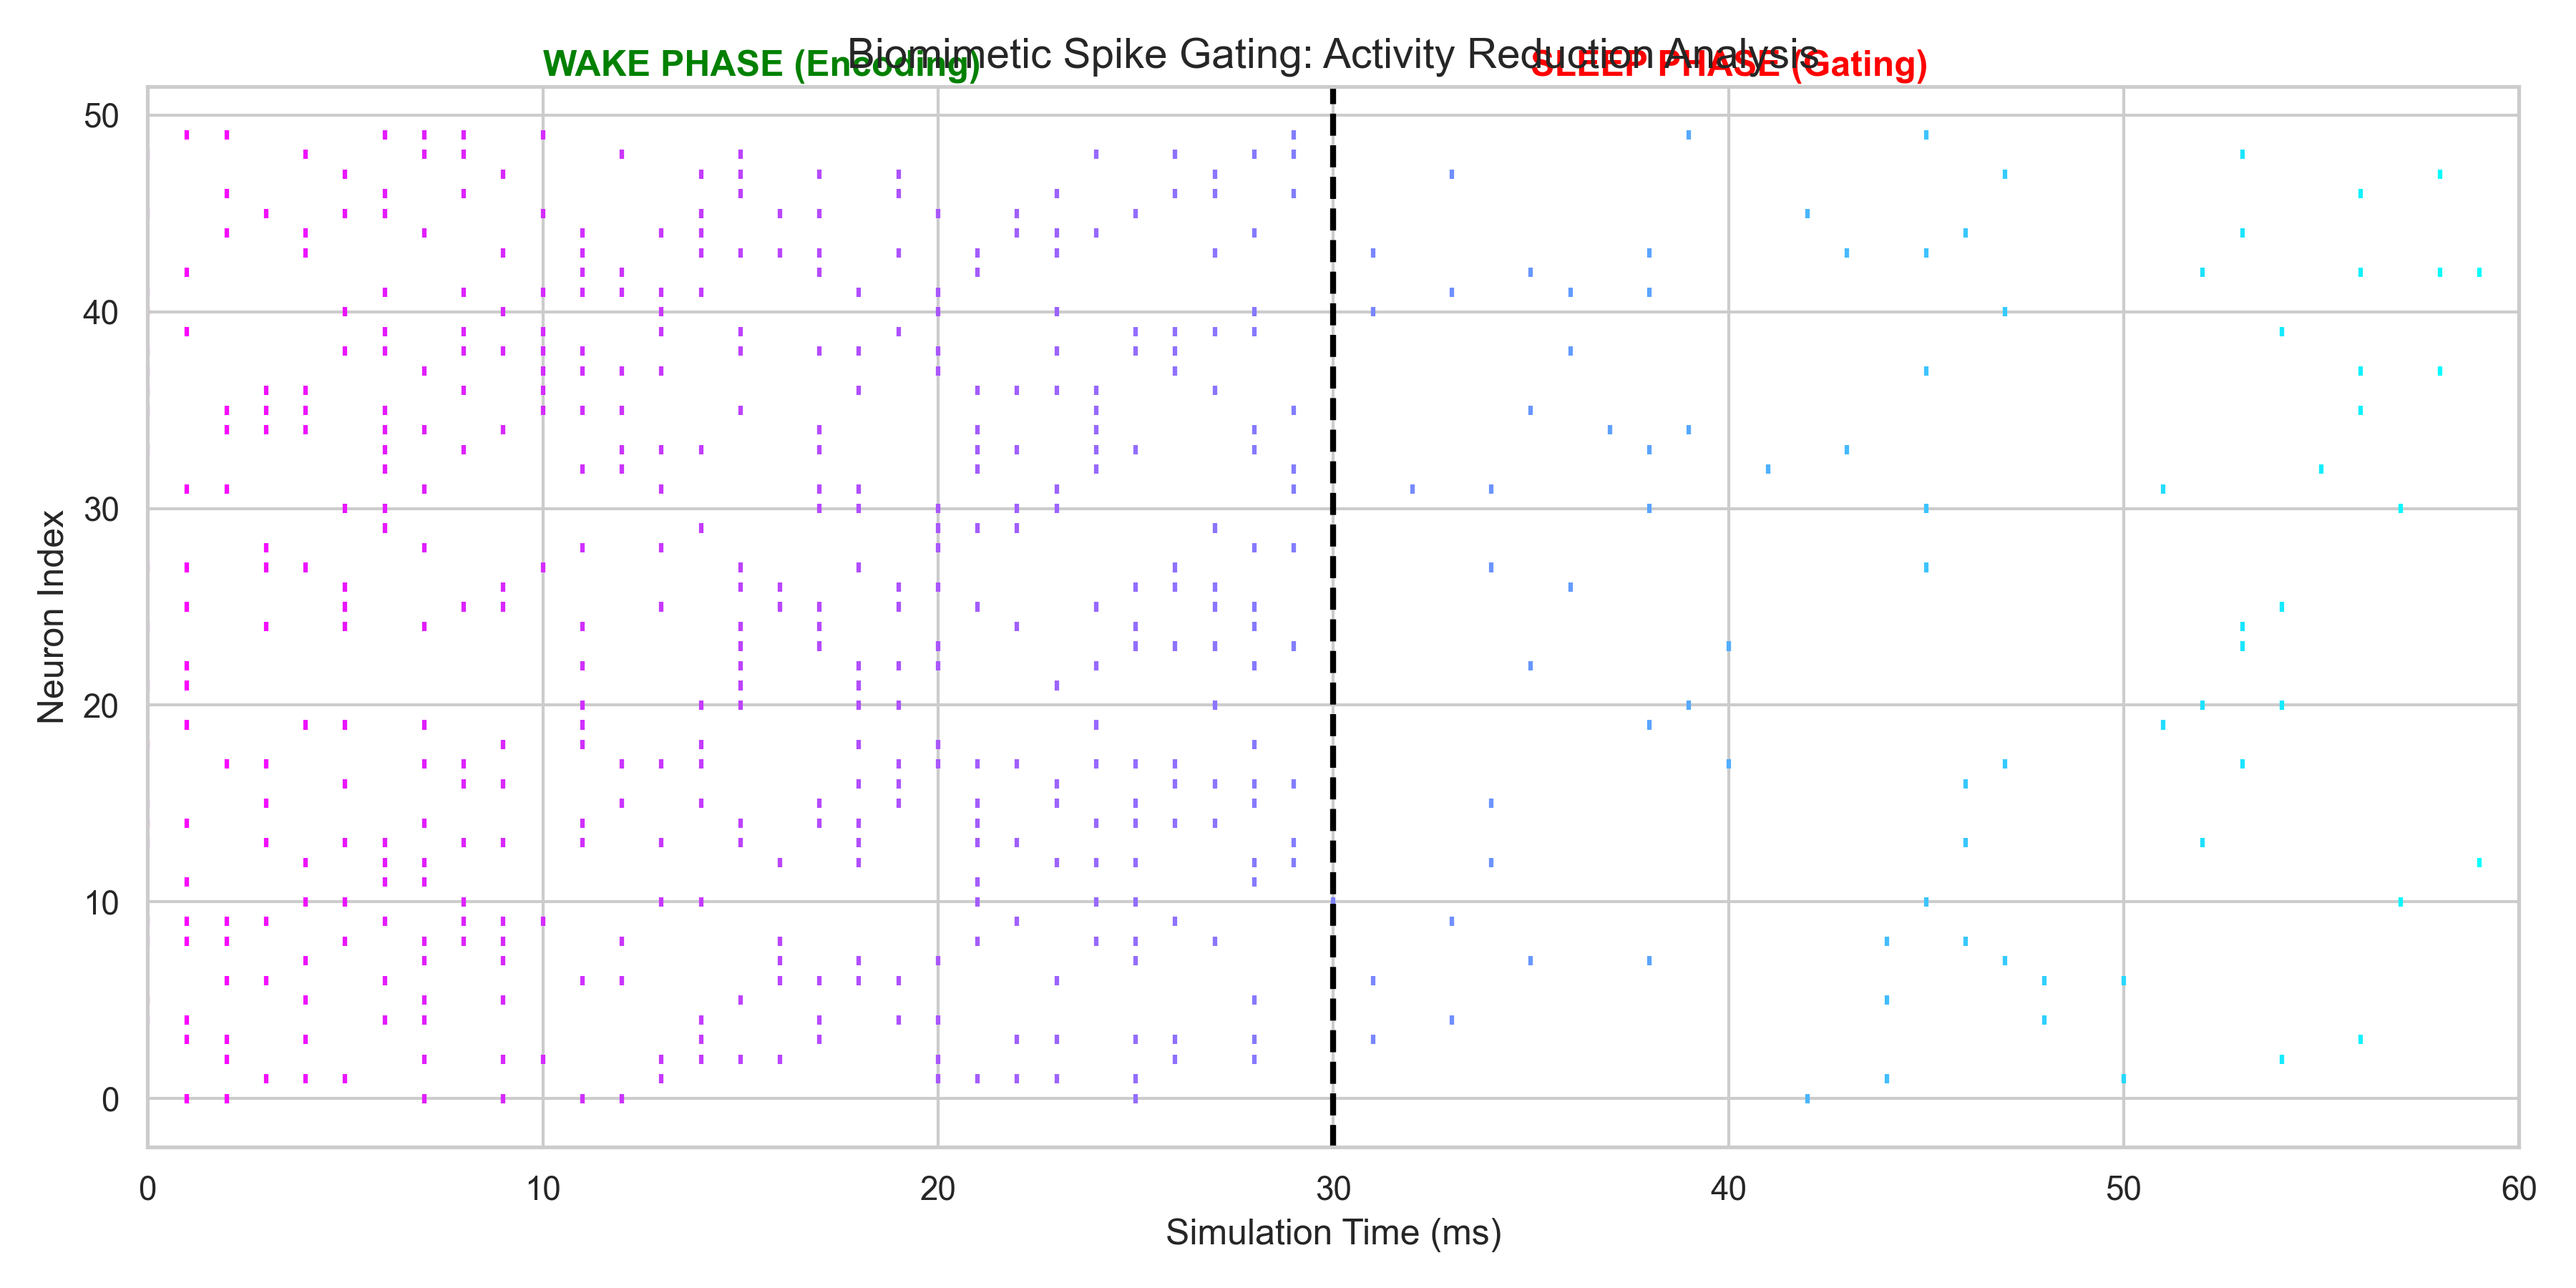
\includegraphics[width=0.92\linewidth]{figures/page5_img1_rotated.png}
\caption{Raster plot extracted from the source PDF. The dashed line marks the onset of the sleep phase; activity becomes markedly sparser afterward.}
\label{fig:nsn-raster}
\end{figure}

\begin{figure}[t]
\centering
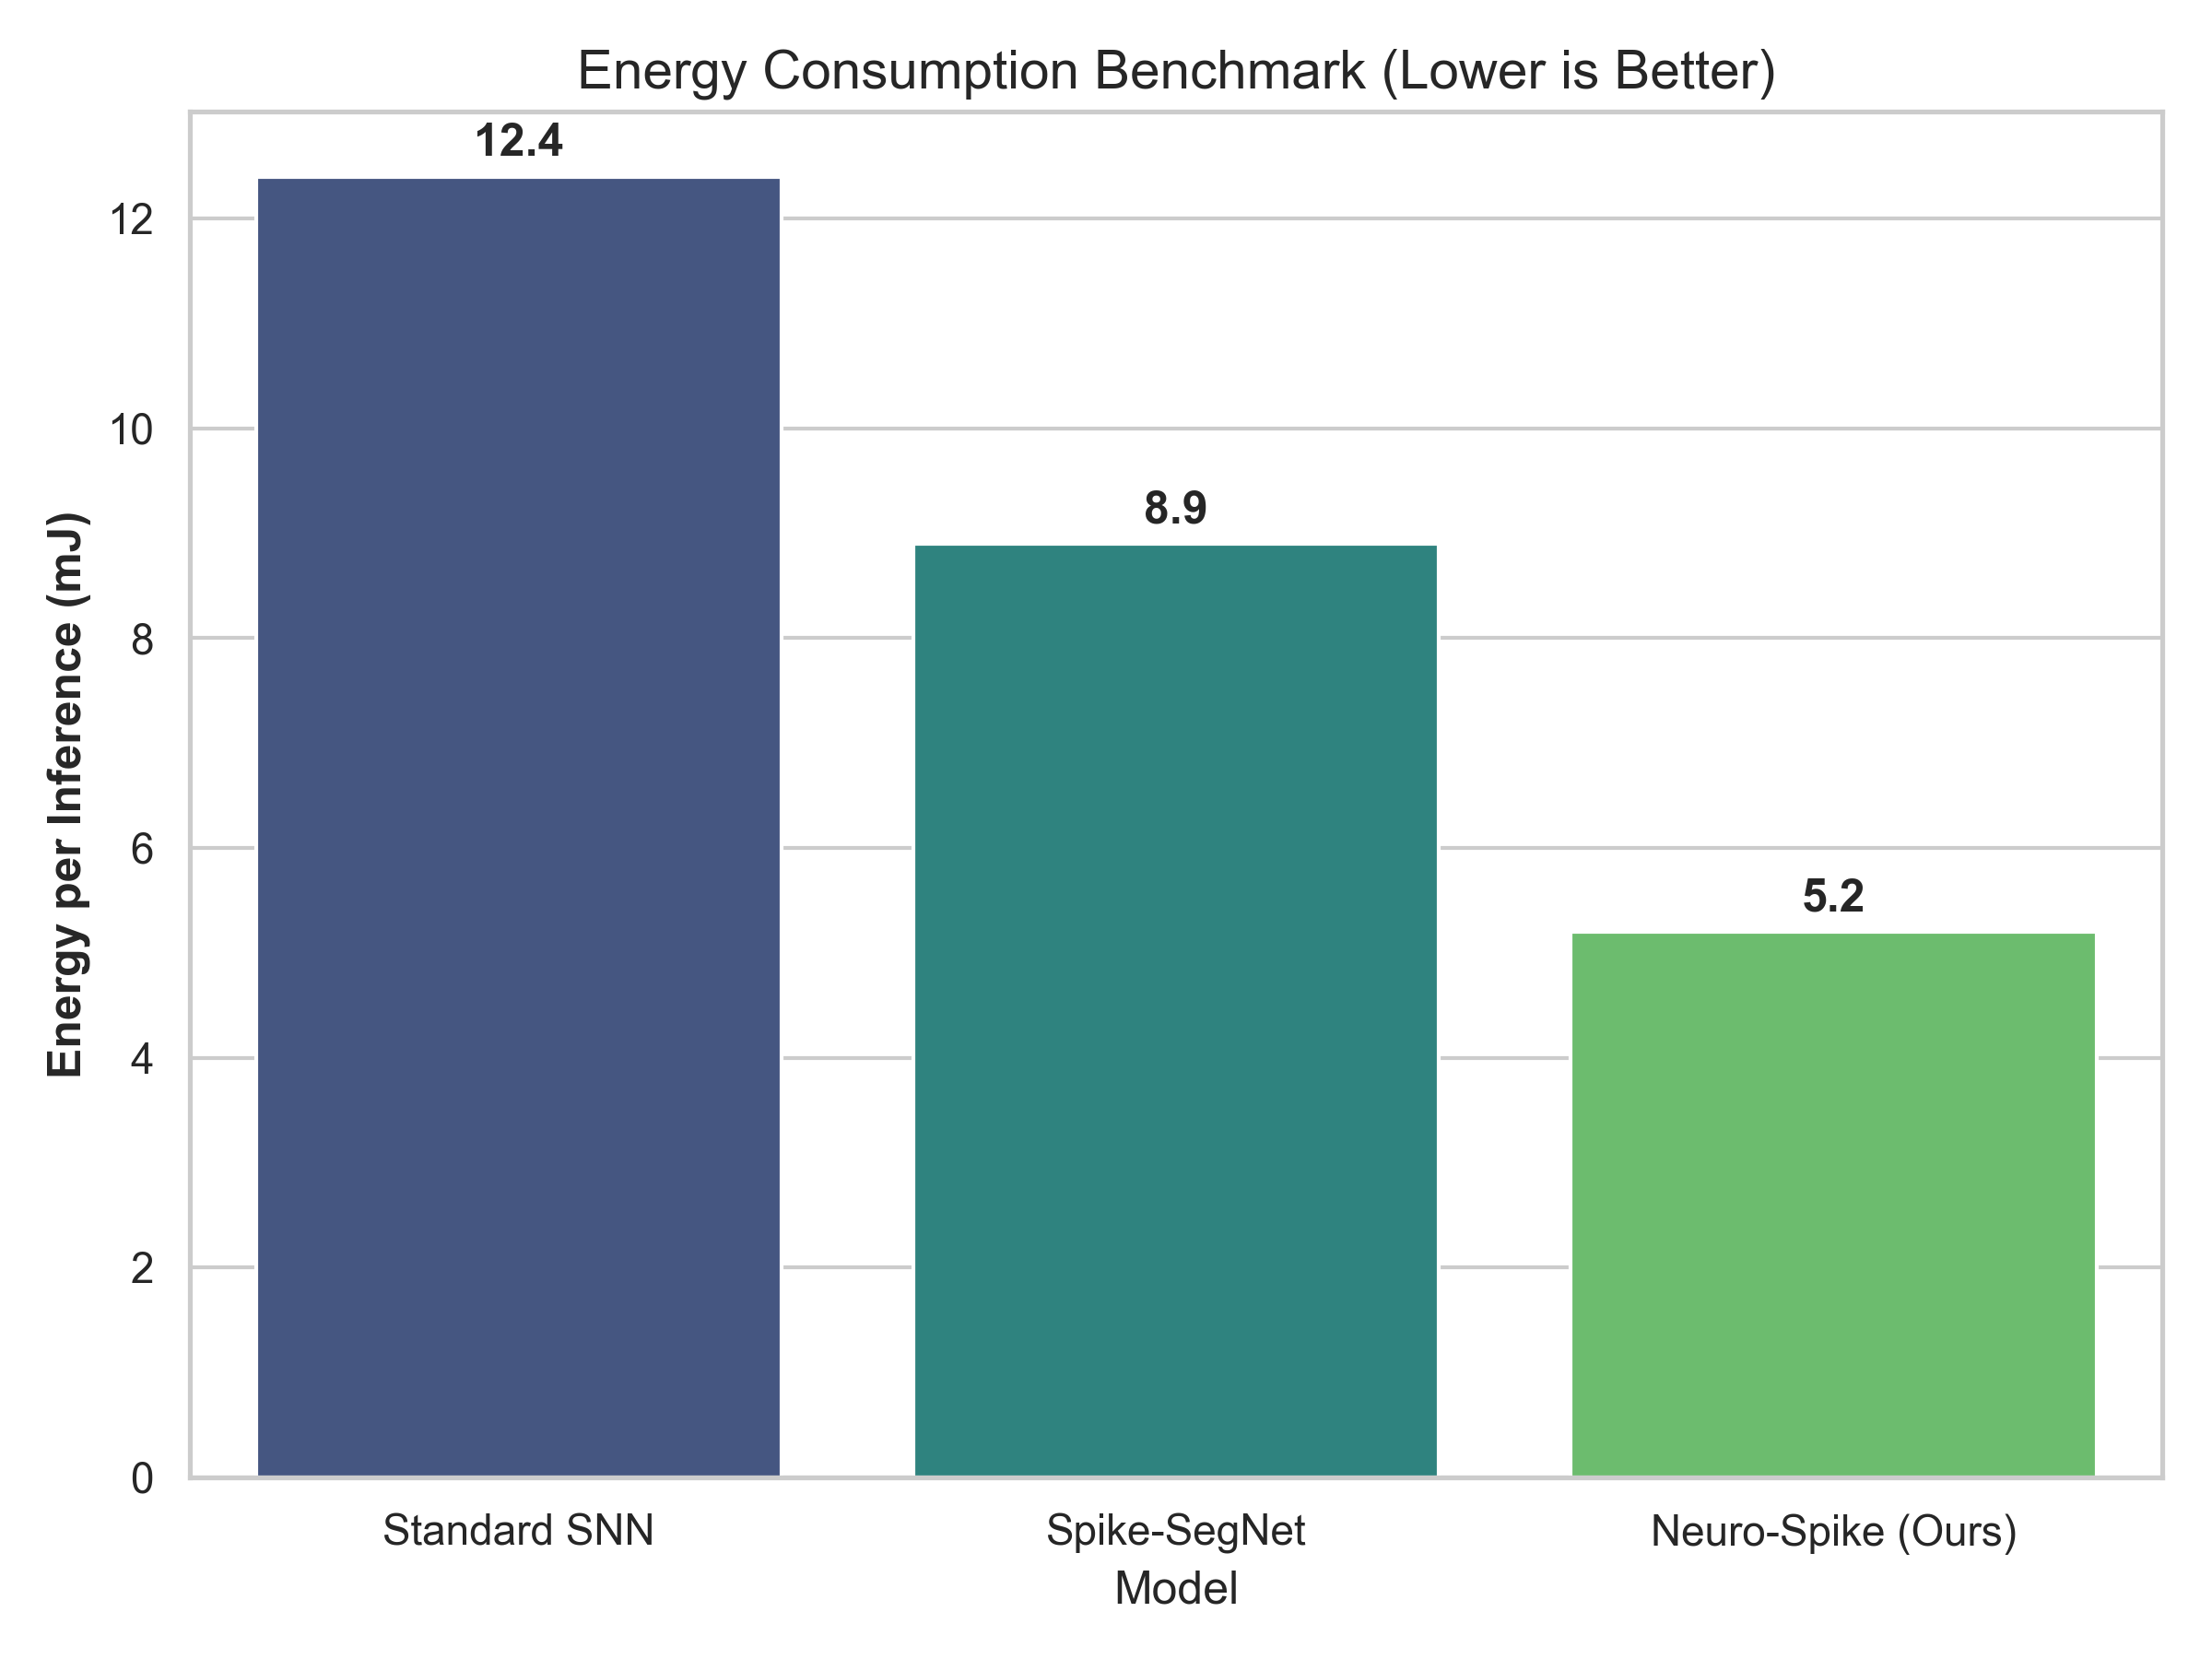
\includegraphics[width=0.82\linewidth]{figures/page6_img1.png}
\caption{Energy comparison extracted from the source PDF. The gated model is reported as the lowest-energy configuration among the compared variants.}
\label{fig:nsn-energy}
\end{figure}

\section{Discussion}
The appealing feature of Neuro-Spike SegNet is that it treats redundancy as something the dynamics can actively suppress, not merely something training hopes will disappear. That is a stronger systems claim than generic sparsity regularization. The wake phase accumulates enough evidence to establish a dense segmentation hypothesis, while the sleep phase functions as a controlled consolidation stage that forces only high-confidence structures to remain metabolically active.

This idea also gives the architecture a clearer niche within spiking vision research. Existing efficiency improvements often act through weight learning, surrogate gradients, or architectural compression \citep{fang2021deep,neftci2019surrogate}. The present mechanism instead intervenes at inference time by changing the physical interpretation of the neuron. That distinction is publishable in principle because it leads to different falsifiers and different deployment knobs.

\section{Limitations and Future Work}
The current manuscript is still limited by its dependence on source-reported experiments rather than a fresh replication package. Several gaps remain:
\begin{enumerate}[leftmargin=*]
\item the energy model is proxy-based rather than hardware-measured,
\item the reported evidence emphasizes static scenes more than dynamic ones,
\item the global gate may be too coarse for heterogeneous scenes, and
\item the segmentation benchmark needs broader dataset reporting beyond the summarized examples.
\end{enumerate}

The next serious step is to reproduce the reported results with explicit code, per-layer spike accounting, and latency measurements. A stronger follow-up would also compare global gating against spatially adaptive gating and against rate-regularized baselines.

\section{Conclusion}
Neuro-Spike SegNet is most interesting when interpreted not as a loose biological metaphor but as a concrete dynamical hypothesis: late-phase spikes in dense spiking segmentation can be selectively suppressed through phase-dependent membrane control. The original PDF provides promising evidence for that claim, and this rebuild organizes it into a more formal manuscript foundation for later experimental expansion.

\section*{Declarations}
\paragraph{Funding} No external funding was received for this work.
\paragraph{Competing interests} The author declares no competing interests.
\paragraph{Data and materials availability} The source manuscript and extracted figure assets used in this paper package are available from the corresponding author upon reasonable request.
\paragraph{Code availability} The present manuscript is a theory-and-reconstruction package; any supporting analysis scripts used for packaging are available from the corresponding author upon reasonable request.
\paragraph{Author contributions} Aryan Singh Chandel: conceptualization, formalization, analysis, writing---original draft, writing---review and editing.

\bibliographystyle{plainnat}
\bibliography{references}

\end{document}
